\documentclass[fleqn,a4paper,12pt]{article}
\usepackage[top=1in, bottom=1in, left=1in, right=1in]{geometry}



\title{Machine Learning Techniques Homework 4}
\date{}

\setcounter{section}{3}

\usepackage{listings}

\usepackage{amsmath}
\usepackage{amssymb}

\usepackage{graphicx}
\usepackage{caption}
\usepackage{subcaption}
\usepackage{float}


\usepackage{mathspec}
\setmainfont{Noto Serif CJK TC}
% \setmathsfont(Digits,Latin,Greek)[Numbers={Lining,Proportional}]{DejaVu Math TeX Gyre}
\newfontfamily\ZhFont{Noto Serif CJK TC}
\newfontfamily\SmallFont[Scale=0.8]{Droid Sans}
% \newfontfamily\SmallSmallFont[Scale=0.7]{Noto Serif CJK}
\usepackage{fancyhdr}
\usepackage{lastpage}
\pagestyle{fancy}
\fancyhf{}
\rhead{B03902072\ZhFont{江廷睿}}
\lhead{Machine Learning Techniques Homework 4}
\rfoot{\thepage / \pageref{LastPage}}

\usepackage{parskip}

\begin{document}
\maketitle
\thispagestyle{fancy}

\section*{1}

The probability that an example is not sampled by one sampling is $1 - \frac{1}{N}$. Since $pN$ examples are sampled out, the probability of an example is not sampled at all is

\begin{equation*}
  (1 - \frac{1}{N})^{pN} = ((1 - \frac{1}{N})^{N})^{p} = (e^{-1})^{p} = e^{-p}
\end{equation*}

Thus, approximately $e^{-p} N$ examples will not be sampled at all.

\section*{2}

Minimal $E_{in} = 0$. Since to achieve no prediction error, only two of the three tree predicting correctly is required. Let the test data set be $X$, and

\begin{equation*}
  \begin{cases}
    X_1 = \{ x \in X | \text{ $g_1(x)$ is incorrect} \} \\
    X_2 = \{ x \in X | \text{ $g_2(x)$ is incorrect} \} \\
    X_3 = \{ x \in X | \text{ $g_3(x)$ is incorrect} \} \\
  \end{cases}
\end{equation*}

since $E_{out}(g_1) + E_{out}(g_2) + E_{out}(g_3) \le 1$, it is possible that $X_1, X_2, X_3$ are pairwaise disjoint. So if $X_1, X_2, X_3$ are pairwise disjoint, for all $x \in X$, if $x \in X_k$, $x \notin X_{i}$ for $i \in \{1, 2, 3\} \\k$. It implies that for any $x \in X$, at least two of $g_1, g_2, g_3$ will predict correctly. Therefore, $E_{in} = 0$ is attained.

Maximun $E_{out} = 0.375$, which is achieveable only if $X_1 \cup X_2 \cup X_3 = \phi$ to maximize

\begin{equation*}
  E_{out} = \frac{|(X_1 \cap X_2) \cup (X_2 \cap X_3) \cup (X_1 \cap X_3)|}{|X|}
\end{equation*}

And also since an error prediction on $x$ requires two $g$ that predict incorrectly, thus the constraint becomes

\begin{equation*}
  \begin{cases}
    X_3 \subset X_1 \cup X_2 \\
    X_3 \cap (X_1 \cap X_2) = \phi 
  \end{cases}
\end{equation*}

So the $E_{out}(G) = (|X_3| + |X_1 \cap X_2|) / |X|$ where $|X_3| = 0.35 |X|$, and

\begin{equation*}
  \begin{aligned}
    & \text{maximize} && |X_1 \cap X_2| \\
    & \text{subject to} && 
    \begin{cases}
      X_3 \subset X_1 \cup X_2 \\
      X_3 \cap (X_1 \cap X_2) = \phi 
    \end{cases}
  \end{aligned}
\end{equation*}

is to

\begin{equation*}
  \begin{aligned}
    & \text{maximize} && |X_4| \\
    & \text{subject to} && 
    \begin{cases}
      X_4 \subset X_1, X_2 \\
      X_3 \subset (X_1 \setminus X_4) \cup (X_2 \setminus X_4) \\
      X_3 \cap X_4 = \phi 
    \end{cases}
  \end{aligned}
\end{equation*}

that is 

\begin{equation*}
  \begin{aligned}
    & \text{maximize} && |X_4| \\
    & \text{subject to} && 
    \begin{cases}
      |X_3| \leq (|X_1| - |X_4|)  + (|X_2| - |X_4|) \\
    \end{cases}
  \end{aligned}
\end{equation*}

we get the maximum $|X_4| = 0.025$. Thus, maximum $E_{out}(G) = 0.35 + 0.025 = 0.375$.

\section*{3}

Let $X$ be the test example set, and

\begin{equation*}
  X_i = \{x \in X | \text{$g_i(x)$ is incorrect} \}
\end{equation*}

Let

\begin{equation*}
  W_p = \bigcap_{i \in p} X_i
\end{equation*}

where $p \in P$ and

\begin{equation*}
  P = \{ p \subset \{1, 2, 3, \cdots, K\} | |p| = \frac{K + 1}{2} \}
\end{equation*}

So for $x \in W_p$, $x$ is predicted incorrectly by $\frac{K + 1}{2}$ hypothesises $g$s, and thus predicted incorrectly by $G$. Therefore,

\begin{align*}
  &E_{out}(G) \cdot |X| \\
  =& \lvert \bigcup_{p \in P} W_p \rvert \\
  =& \sum_{p \in P} |W_p| - \sum_{p_1, p_2 \in P; p_1 \ne p_2} |W_{p_1} \cap W_{p_2}| + \sum_{p_1, p_2, p_3 \in P; p_1 \ne p_2 \ne p_3 \ne p_1} |W_{p_1} \cap W_{p_2} \cup W_{p_3}| \cdots
\end{align*}

Since if $\{ W_p | p \in P\}$ are not pairwise disjoint,

\begin{equation*}
- \sum_{p_1, p_2 \in P; p_1 \ne p_2} |W_{p_1} \cap W_{p_2}| + \sum_{p_1, p_2, p_3 \in P; p_1 \ne p_2 \ne p_3 \ne p_1} |W_{p_1} \cap W_{p_2} \cup W_{p_3}| \cdots < 0
\end{equation*}

$E_{out}(G) \cdot |X|$ is upper bounded

\begin{equation*}
  E_{out}(G) \cdot |X| = \lvert \bigcup_{p \in P} W_p \rvert \leq \sum_{p \in P} |W_p| 
\end{equation*}

And we know that when $\{ W_p | p \in P\}$ are pairwise disjoint

\begin{align*}
  \sum_{p \in P} |W_p|
  &= \lvert \bigcup_{p \in P} W_p \rvert \\
  &= \lvert \{ x \in W_p \text{ for some $p$ } \} \rvert \\
  &= \lvert \{ x | \text{$x$ in $\frac{K + 1}{2}$ sets ($X_i, \forall i \in p$) that contain $x$} \} \rvert \\
  &= \frac{2}{K + 1} \sum_{k=1}^{K} |X_k| \\
  &= \frac{2}{K + 1} \sum_{k=1}^{K} |X| e_k
\end{align*}


Therefore,

\begin{equation*}
  E_{out}(G) \leq \frac{2}{K + 1} \sum_{k=1}^{K} e_k
\end{equation*}

\section*{4}

To solve

\begin{equation*}
  \min_{\eta} \sum_{n=1}^N ((y_n - s_n) - \eta g_1(x_n))^2  =   \min_{\eta} \sum_{n=1}^N (y_n - 2 \eta )^2
\end{equation*}

Let

\begin{align*}
  \frac{\partial}{\partial \eta} \sum_{n=1}^N (y_n - 2 \eta)^2 
  =& \sum_{n=1}^N -4 (y_n - 2 \eta) = 0
\end{align*}

Get

\begin{equation*}
  \alpha_1 = \eta = \frac{\sum_{n=1}^N y_n}{2N} 
\end{equation*}

Thus

\begin{equation*}
  s_n = \alpha_1 g_1(x_n) = \frac{\sum_{n=1}^N y_n}{2N} \cdot 2 = \frac{\sum_{n=1}^N y_n}{N}
\end{equation*}

\section*{5}


\section*{6}

A general polynomial regression problem is to find an optiomal $w$ that minimizes

\begin{equation*}
  \lVert y - g(z) \rVert^2 = \lVert y - w^T z \rVert^2
\end{equation*}

where

\begin{equation*}
z_n = (1, x_n, x_n^2, x_n^3, \cdots, x_n^k)
\end{equation*}

for a $k$-degree polynomial gregression. ($x_n^k$ is elementwise power of $x_n$.)

So the optimal $w$ satisfies

\begin{equation*}
  \frac{\partial}{\partial w} \lVert y - w^T z \rVert^2 = 2z^T(y - w^T z) = 0
\end{equation*}

where $w^Tz = g(z)$ and since the first row of $z^T$ is an all $1$ vector, therefore we have

\begin{equation*}
  1^T(y - g(z)) = 1^T y - 1^T g(z) = 0
\end{equation*}

That is

\begin{equation*}
  \sum_{n=1}^N y_n = \sum_{n=1}^N g(x_n)
\end{equation*}

So to find minimal $\eta$, let

\begin{equation*}
  \frac{\partial}{\partial \eta} \sum_{n=1}^{N} (y_n - \eta g(x_n))^2 = \sum_{n=1}^N -2 g(x_n) (y_n - \eta g(x_n)) = 0
\end{equation*}

Get

\begin{equation*}
  \eta = \frac{\sum_{n=1}^N y_n}{\sum_{n=1}^N g(x_n)} = 1
\end{equation*}

\section*{7}

Let the optimal $w$ in $g_1, g_2$ be $w_1, w_2$ respectively. Then finding the optimal $g_2$ is to find the optimal $w_2$ that minimize

\begin{equation*}
  \lVert y - s - \eta g_t(x) \rVert^2 = \lVert y - w_1^T z - \eta w_2^T z \rVert^2 = \lVert y - (w_1^T +  \eta w_2^T) z \rVert^2
\end{equation*}

where $z$ is defined as in problem 6. But we know that $w_1$ is the optimal solution that minimizes 

\begin{equation*}
  \lVert y - w_1^T z \rVert^2
\end{equation*}

Thus $w_2 = 0$, and therefore $g_2(x) = 0$

\section*{12}

\begin{figure}[H]
\centering
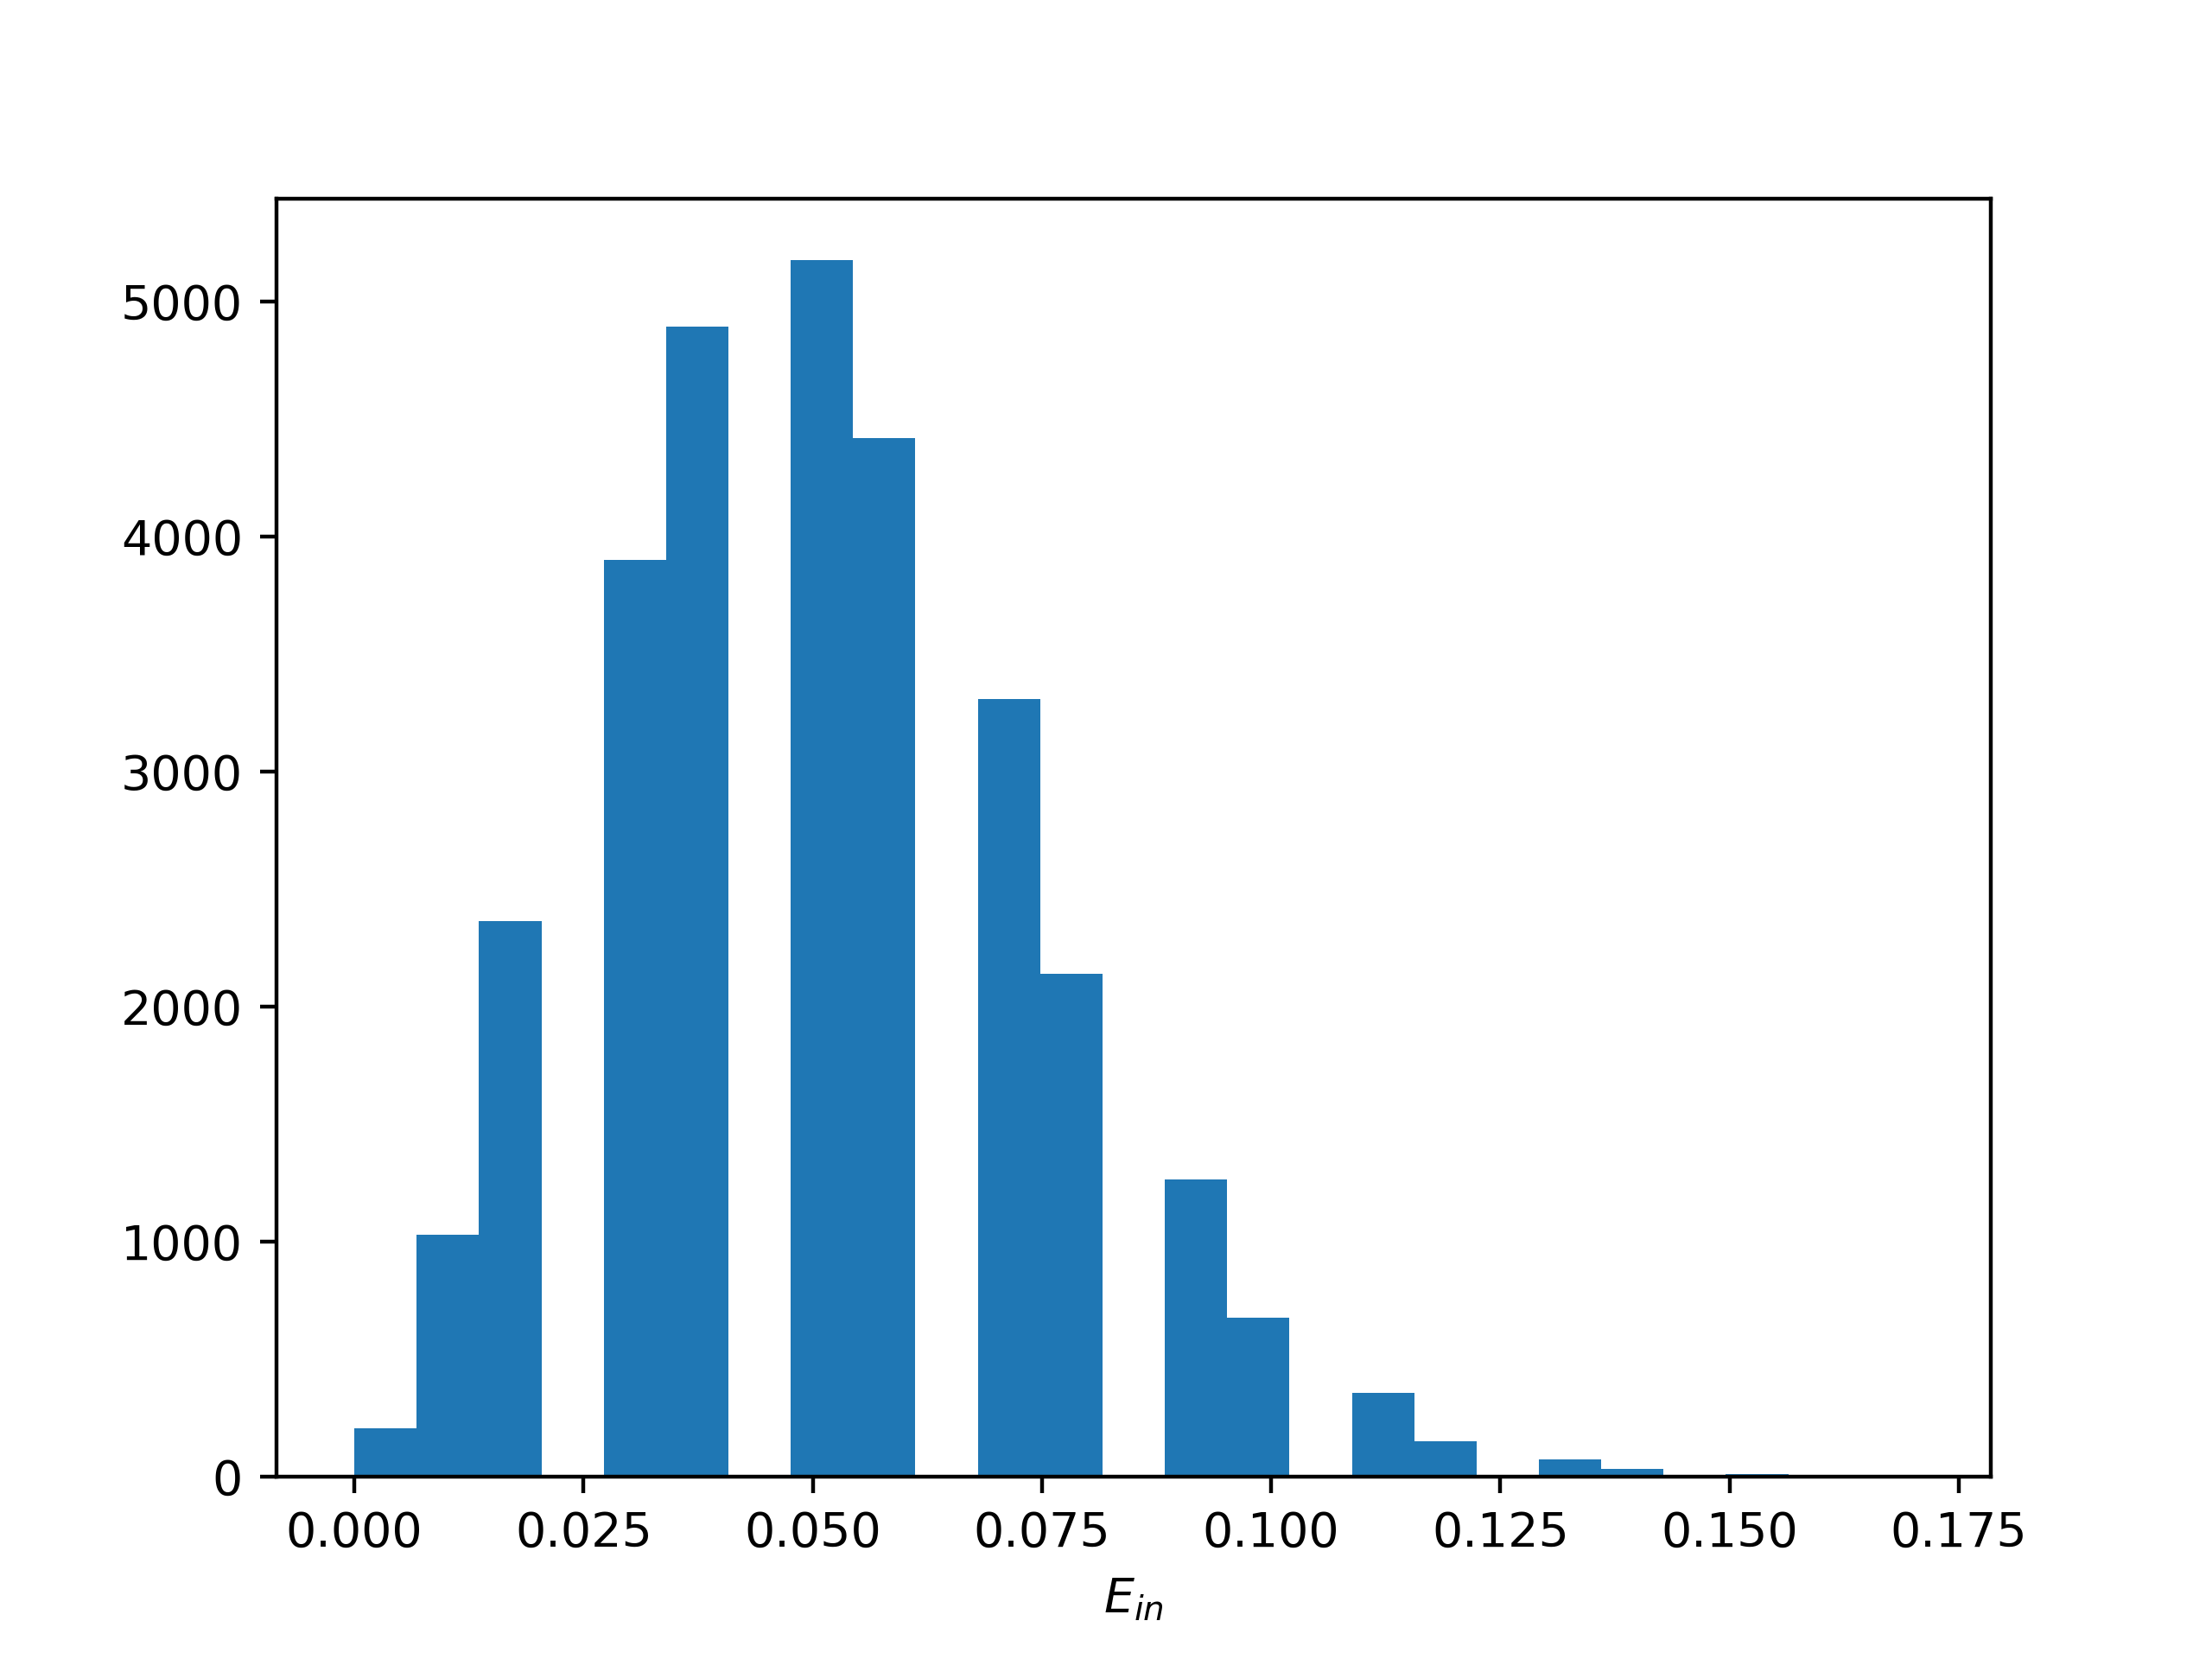
\includegraphics[width=0.75\linewidth]{hist-ein.png}
\caption{$E_{in}$ over 30000 trees}
\label{fig:hist-ein}
\end{figure}

\section*{13}

\begin{figure}[H]
\centering
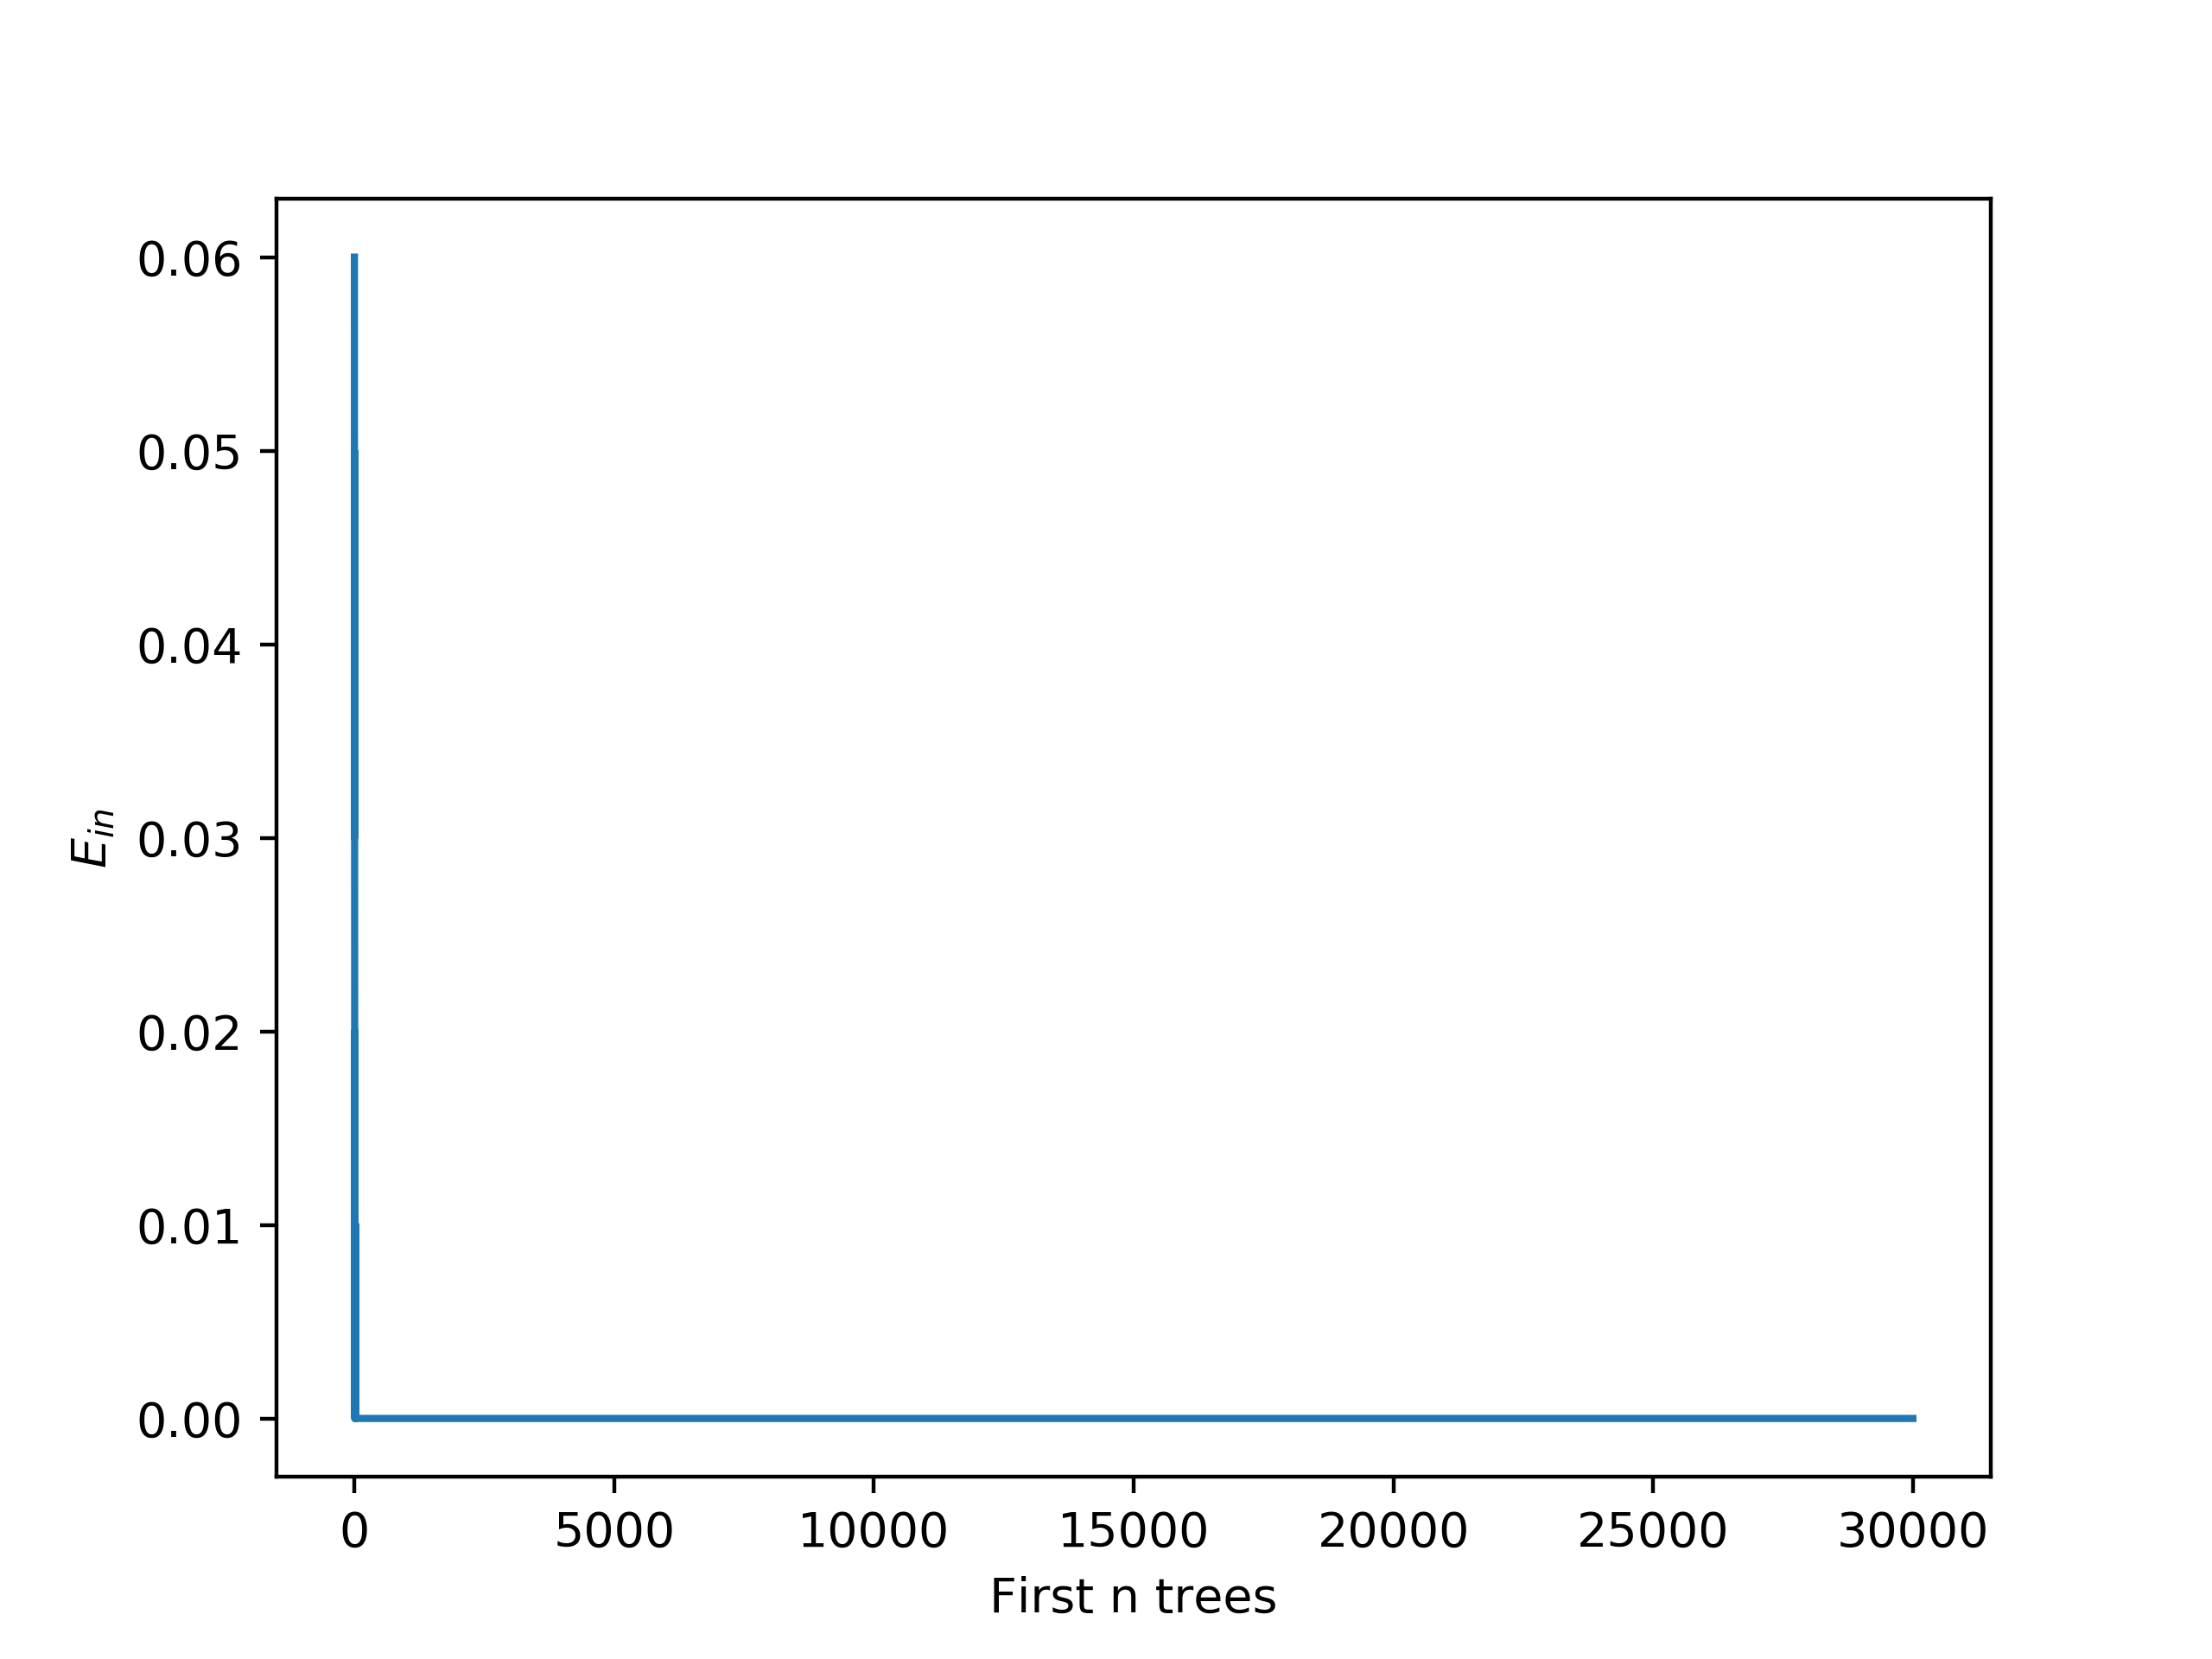
\includegraphics[width=0.75\linewidth]{tree-ein.png}
\caption{$E_{in}$ over 30000 trees}
\label{fig:tree-ein}
\end{figure}

\section*{14}

\begin{figure}[H]
\centering
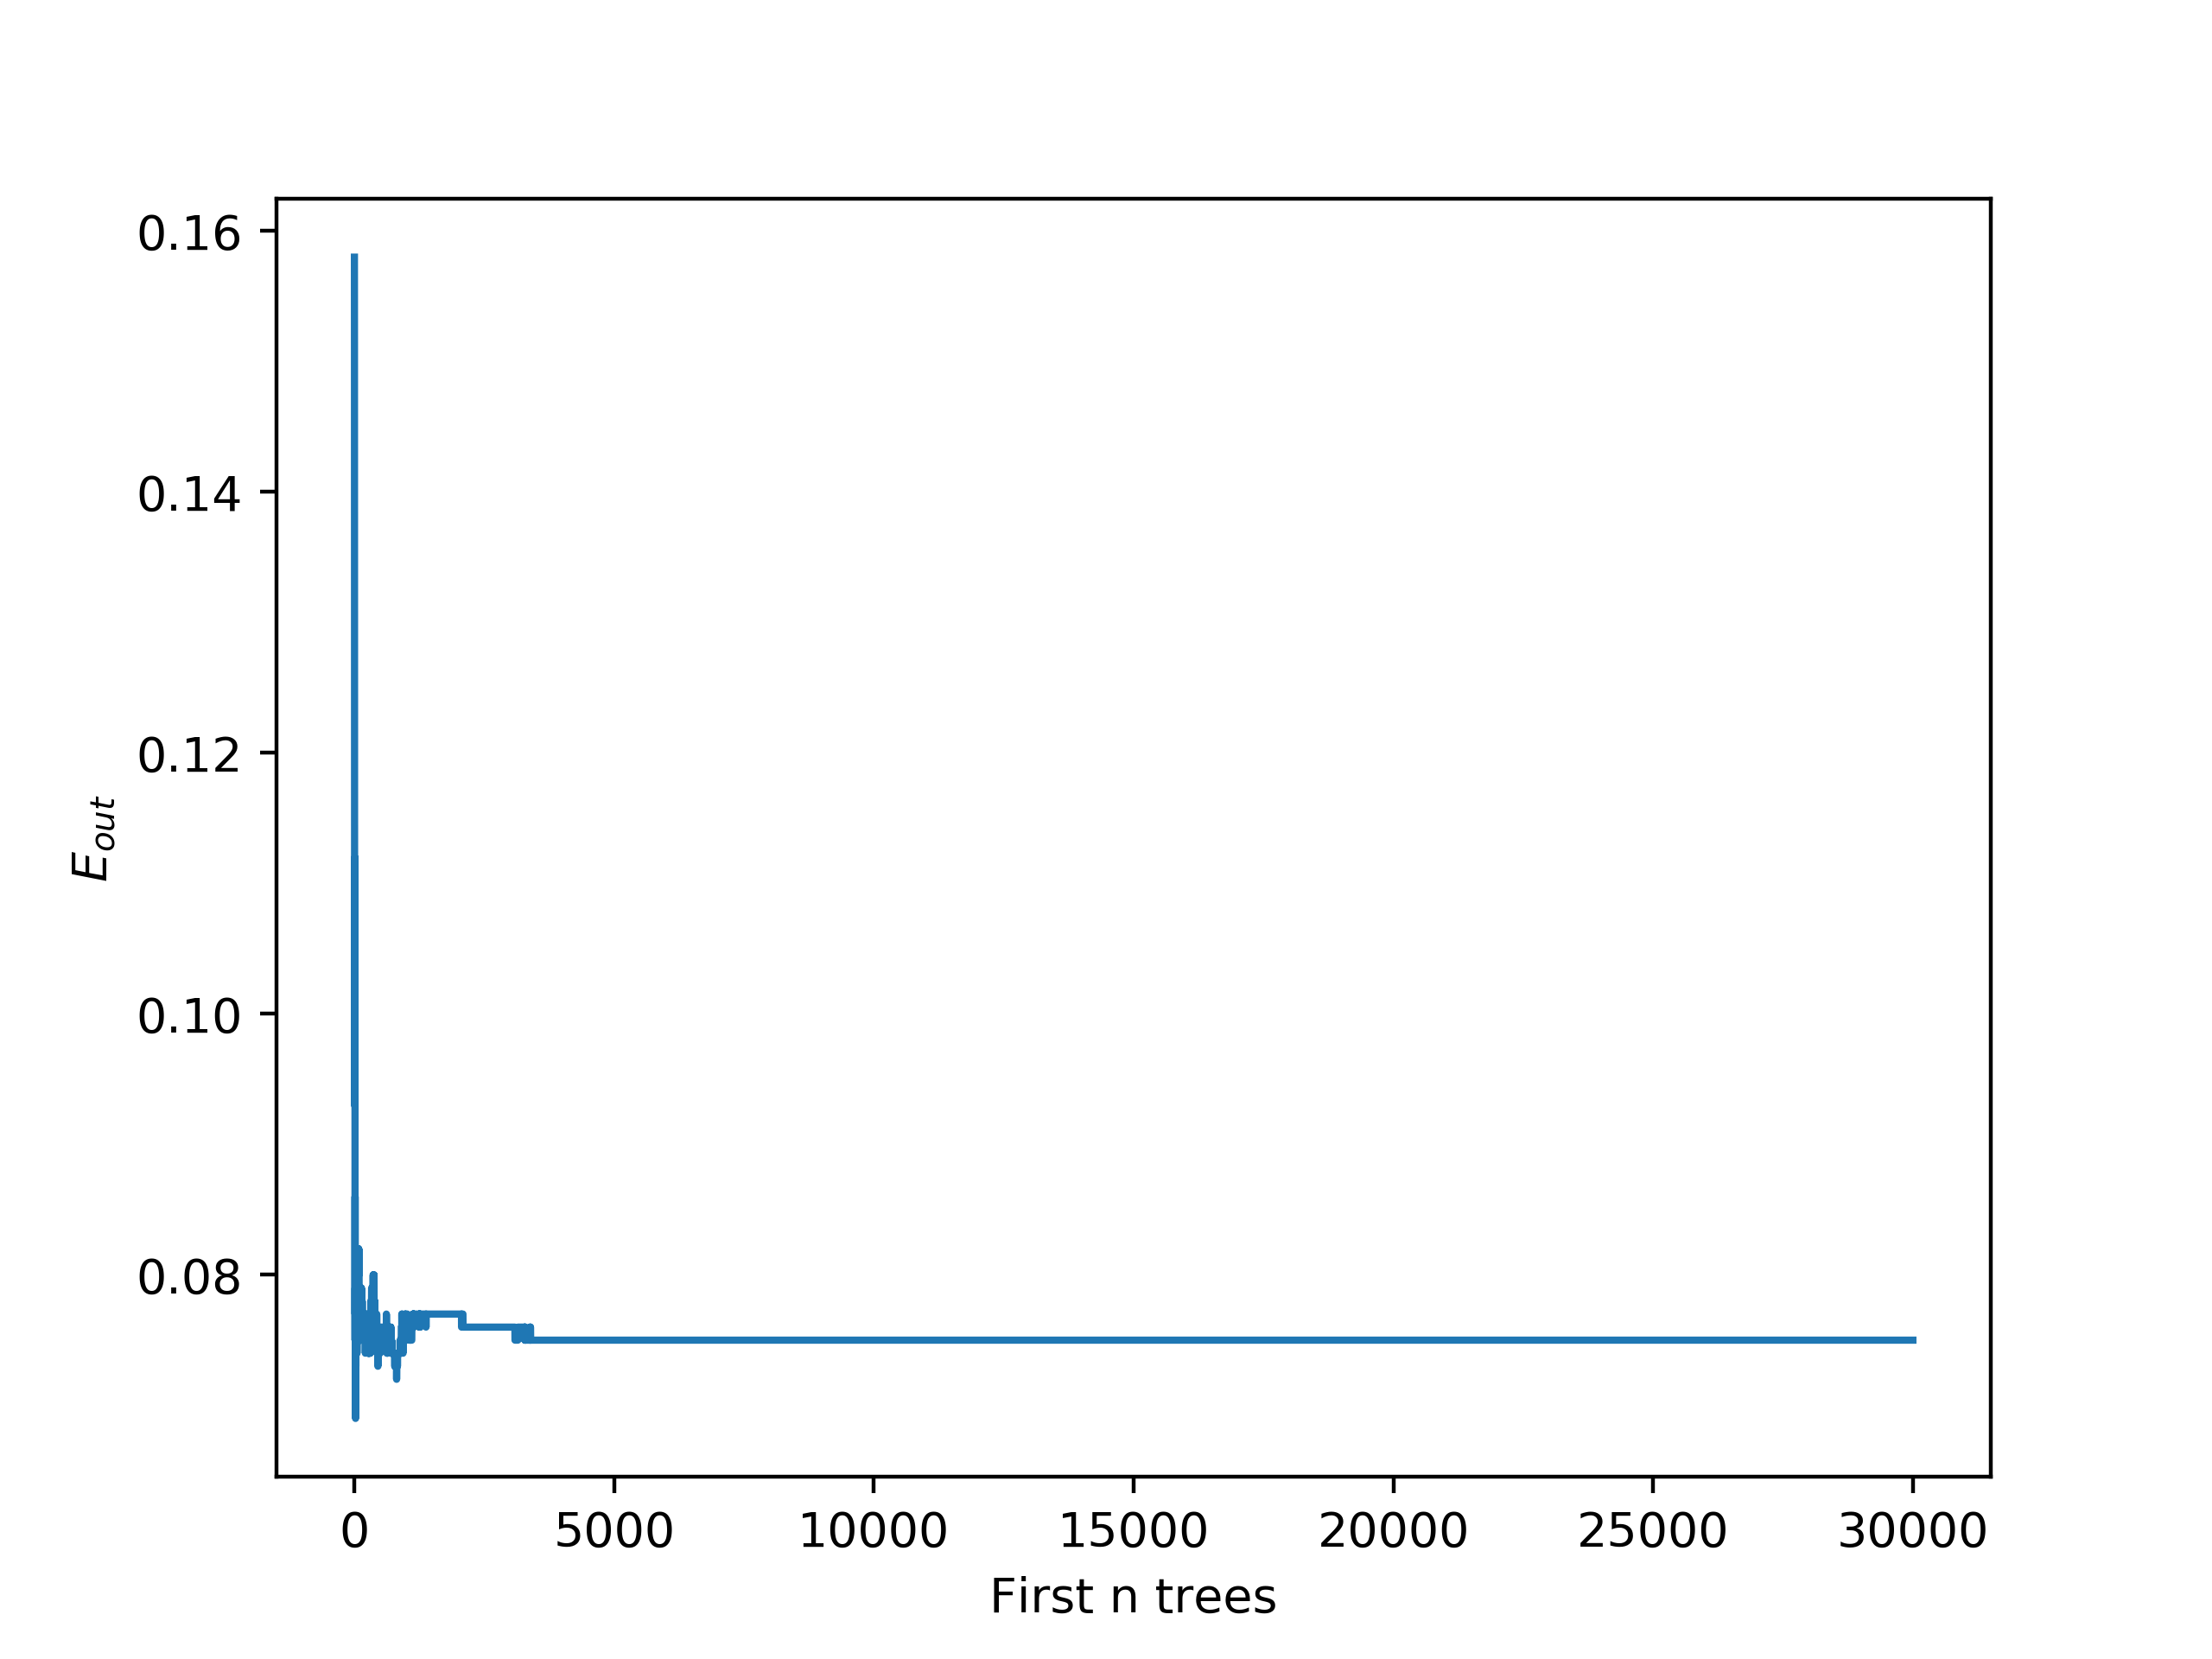
\includegraphics[width=0.75\linewidth]{tree-eout.png}
\caption{$E_{out}$ over 30000 trees}
\label{fig:tree-eout}
\end{figure}

\section*{15}

\begin{figure}[H]
\centering
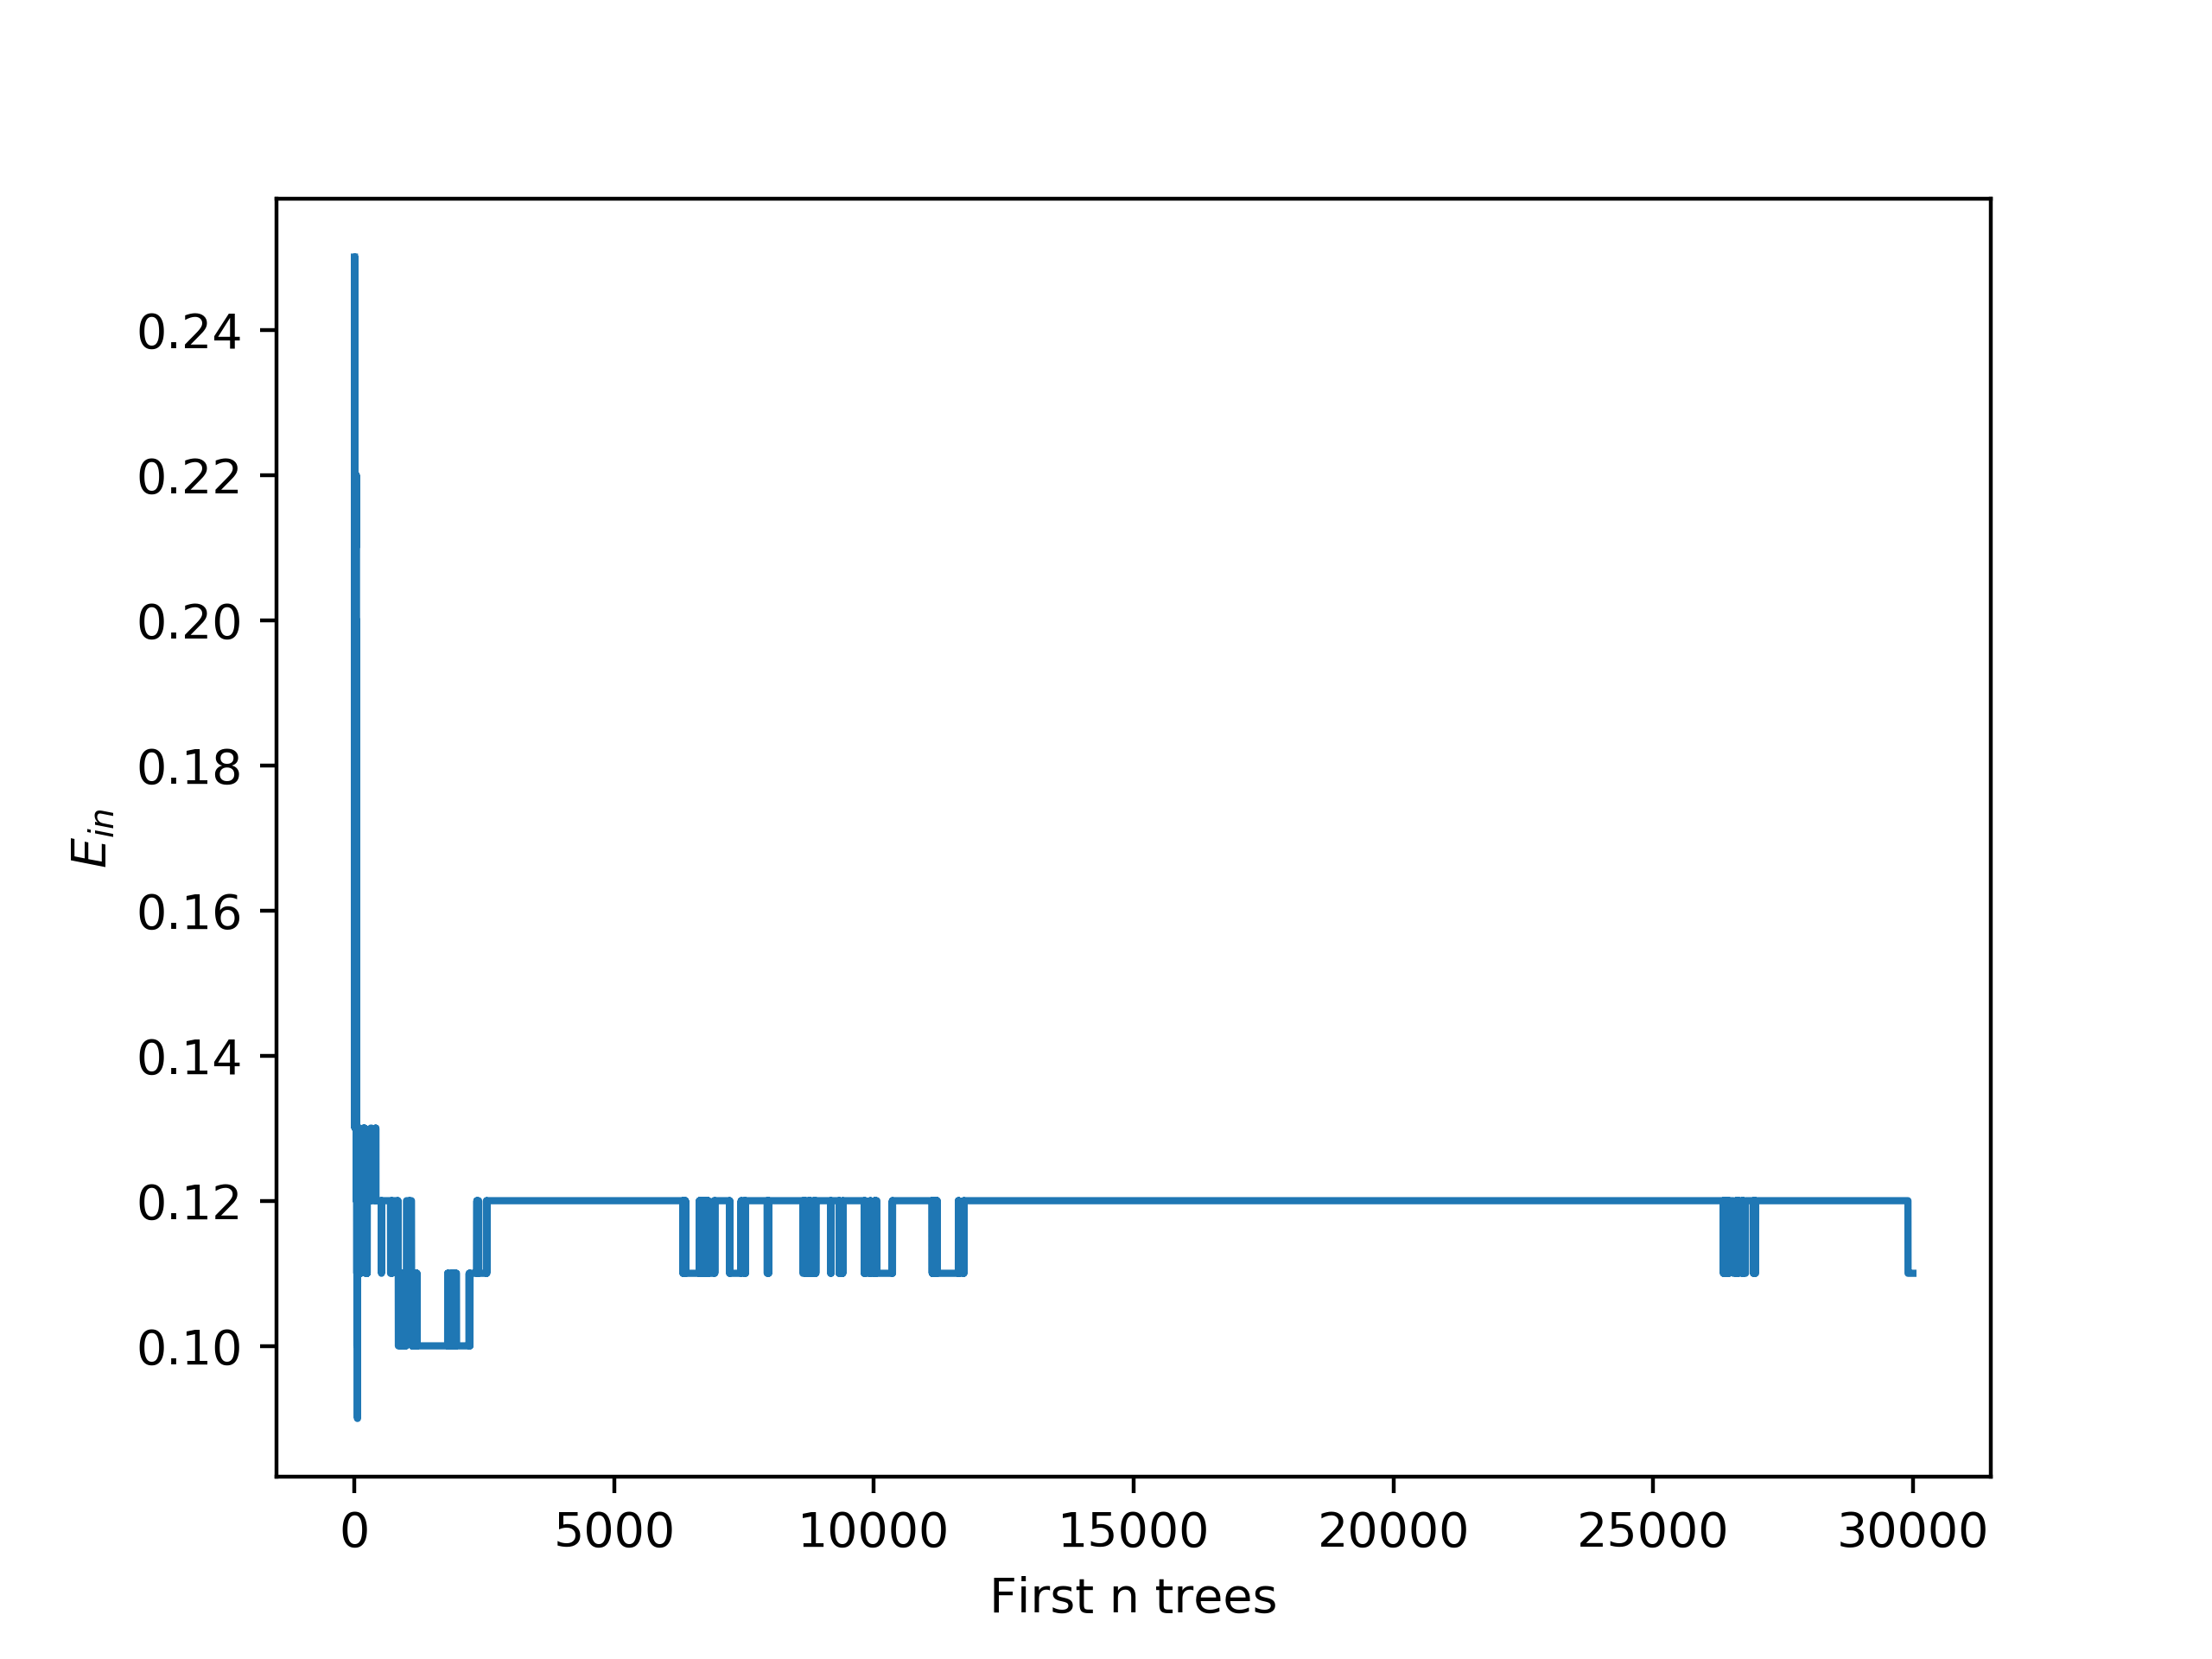
\includegraphics[width=0.75\linewidth]{stump-ein.png}
\caption{$E_{in}$ over 30000 stumps}
\label{fig:stump-ein}
\end{figure}

\section*{16}

\begin{figure}[H]
\centering
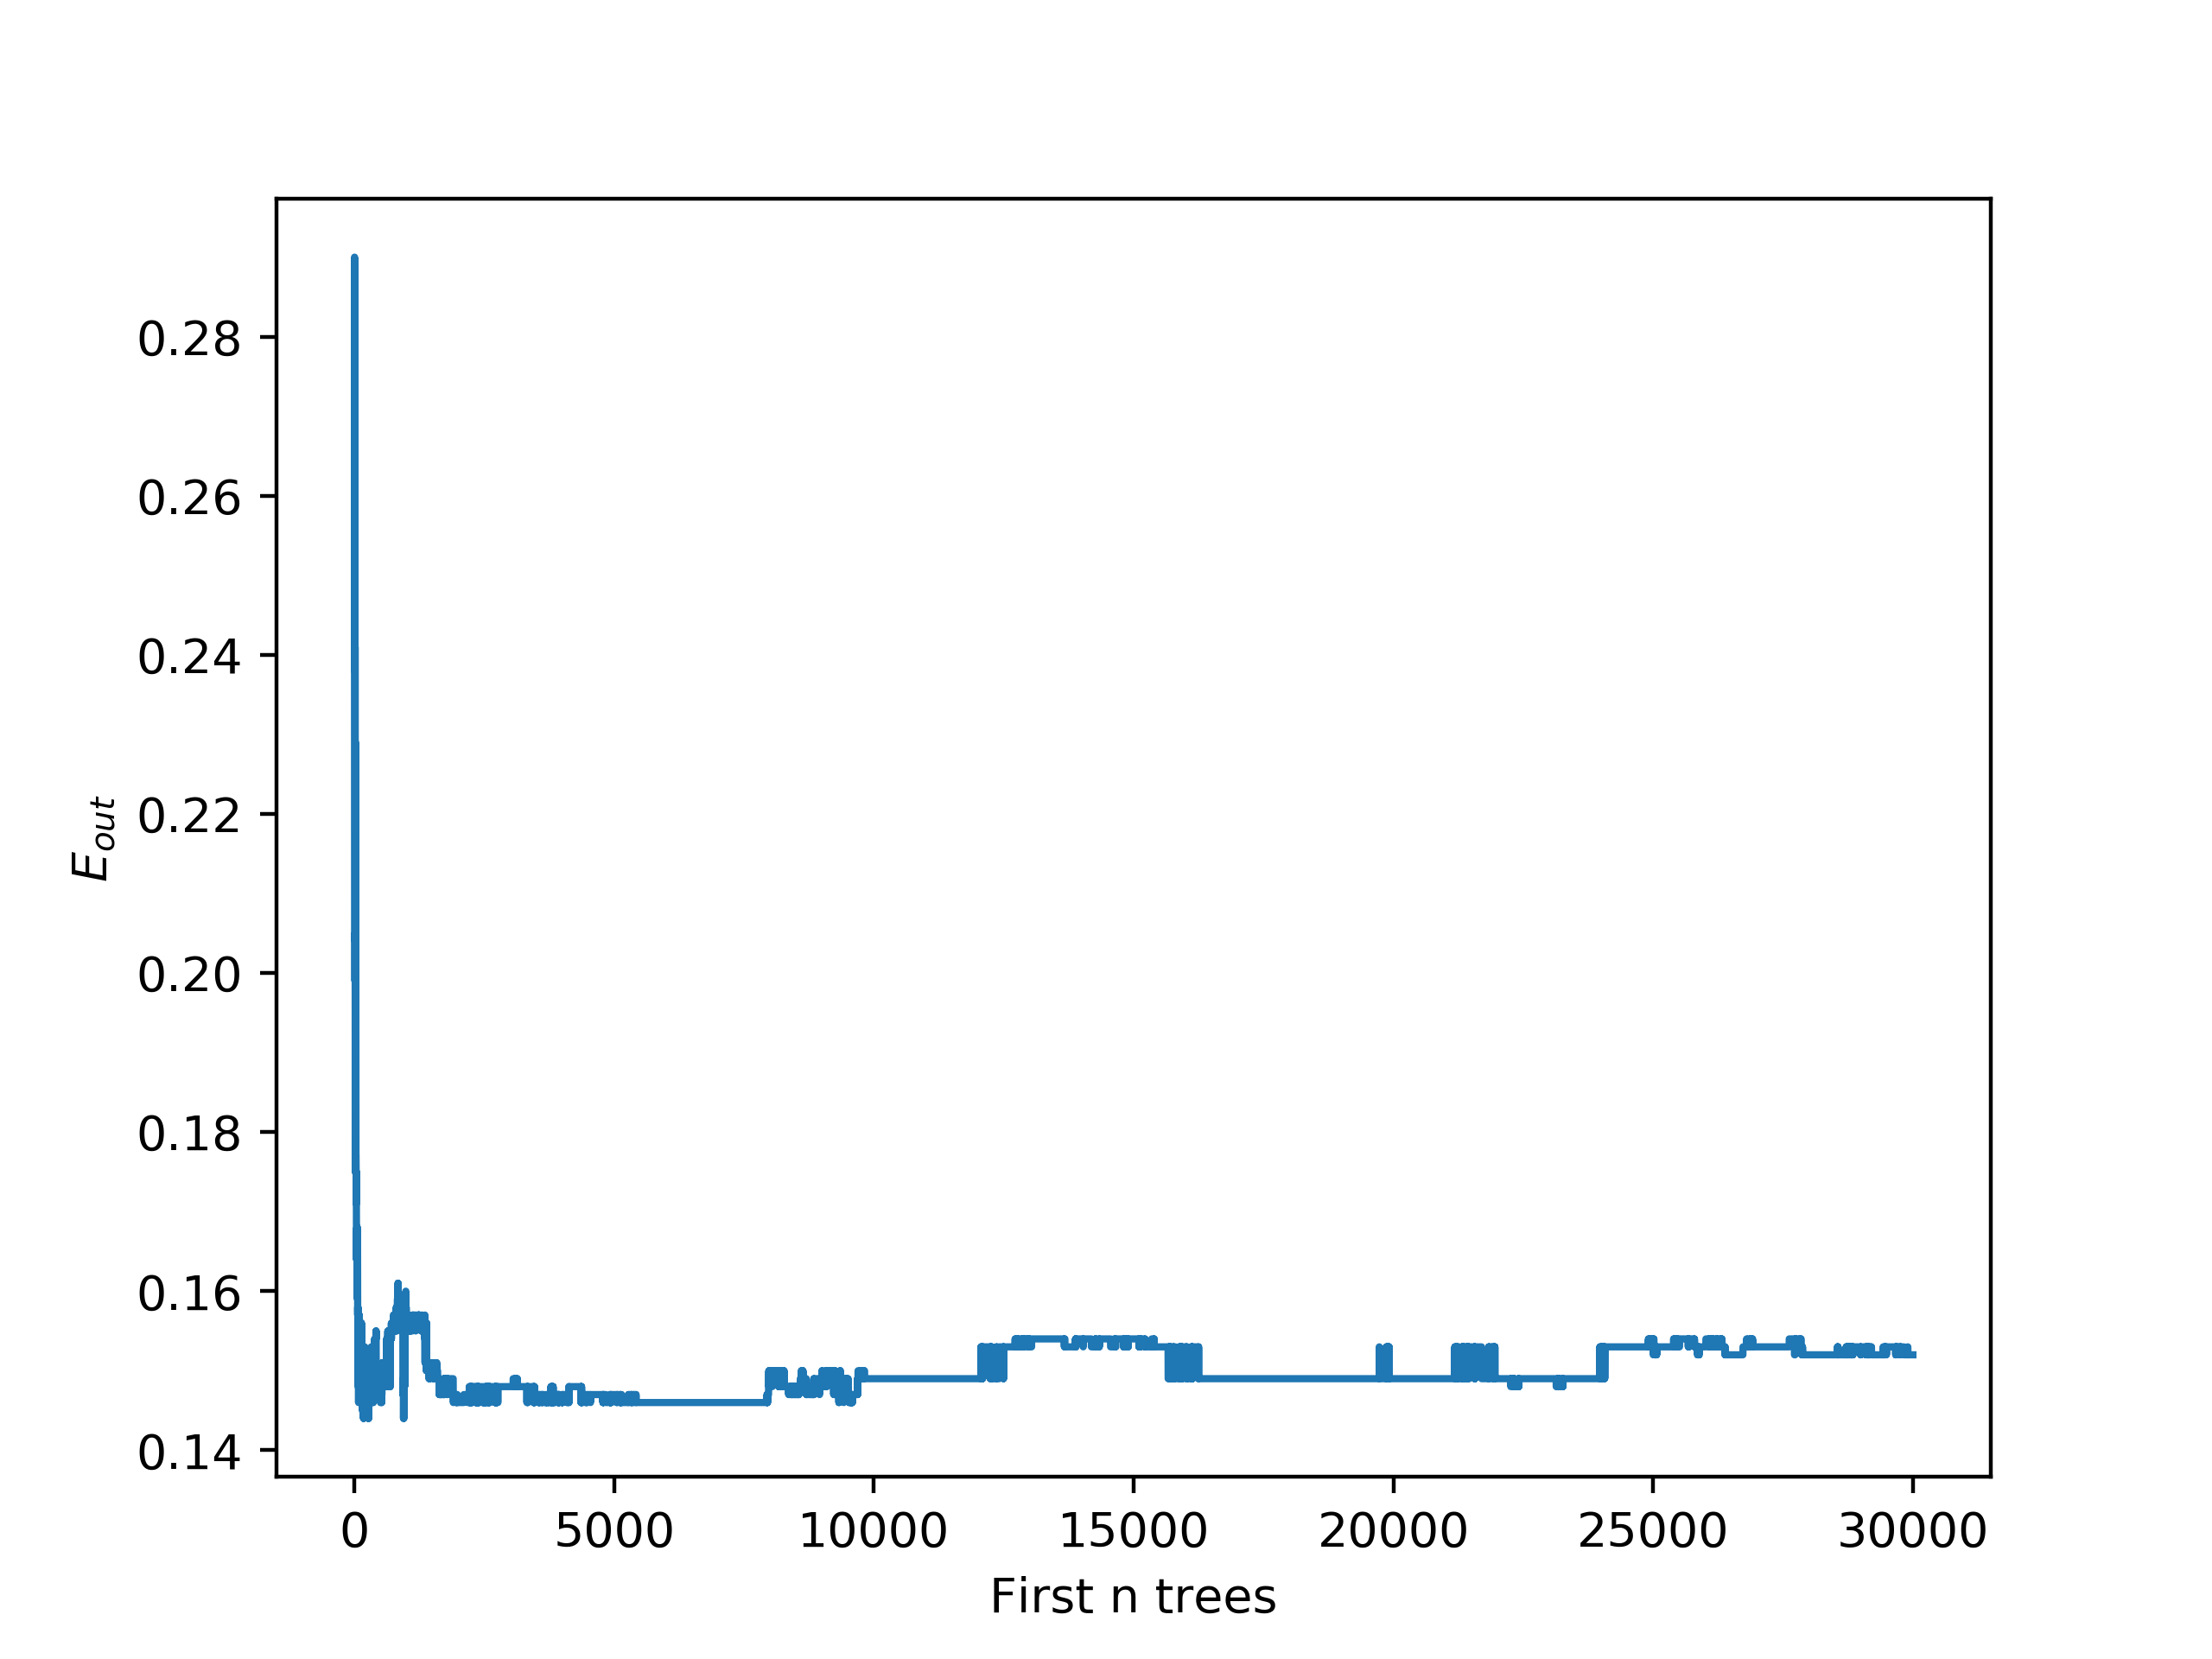
\includegraphics[width=0.75\linewidth]{stump-eout.png}
\caption{$E_{out}$ over 30000 stumps}
\label{fig:stump-eout}
\end{figure}


\end{document}
